\subsection{Hall A Slow Controls}

\subsection{Introduction}
The Hall A base equipment for experiments consists of two general purpose, 
similar, superconducting spectrometers and their associated detector packages as well as
several specific function systems (i.e. cryogenic targets, $\vec{\rm ^3He}$ target, beam current monitors,
ARC energy measurement system, e-p energy measurement systems and so on).
Each of these major systems is, typically, composed of several sub-system levels which need
to be interlocked for protection of human life and/or equipment, monitored for operational status and
commanded to perform various operations so that the system as a whole is able to perform the desired measurement
or function.
Most of these sub-systems have an infrastructure role; they are essential for the correct operation
of the major system of which they are part but, in themselves, are irrelevant for the experimental
physics data being acquired.
An example could be the cryogenics of one of the spectrometer magnets; proper cryogenics filling of the magnets
is absolutely essential for the magnets to operate but, for a given experiment, the relevant quantities are 
the spectrometer momentum and optics produced by the various active magnets and not the cryogenics
levels of each magnet.
The task of monitoring and commanding the infrastructure of the various Hall A systems
falls on a distributed computer system loosely referred to as ``slow controls'' or
``Hall A Controls (HAC)''. 

\subsection{Hall A Controls Overview}
The Hall A distributed control system is based on the 
Experimental Physics and Industrial Control System 
(EPICS)\cite{EPICSwww}%
\htmladdnormallinkfoot{}{\url{http://www.aps.anl.gov/asd/controls/epics/EpicsDocumentation/WWWPages/EpicsDoc.html}}
 architecture.
The basic components of the system are:
\begin{itemize}
\item Operator Interfaces (OPI). These are UNIX based workstations able to run various
EPICS tools like the Motif-based Display Editor/Manager (MEDM) used by the operators
for display and command of the various systems.
\item Input Output Controllers (IOC). These are VME based crates containing a single
board computer with the real-time operating system VxWorks and various I/O modules as well
as interfaces to other I/O busses like serial or GPIB.
\item Boot Servers. These are UNIX based workstations from which the IOCs load the various
software components they need to perform their functions (i.e. operating system, database
of signals to be monitored/commanded, controls algorithms and so on).
\item Local Area Network (LAN). This is the communication path joining the IOCs, OPIs and
the Boot Servers.
\end{itemize}

\begin{figure}[htb]
\begin{center}
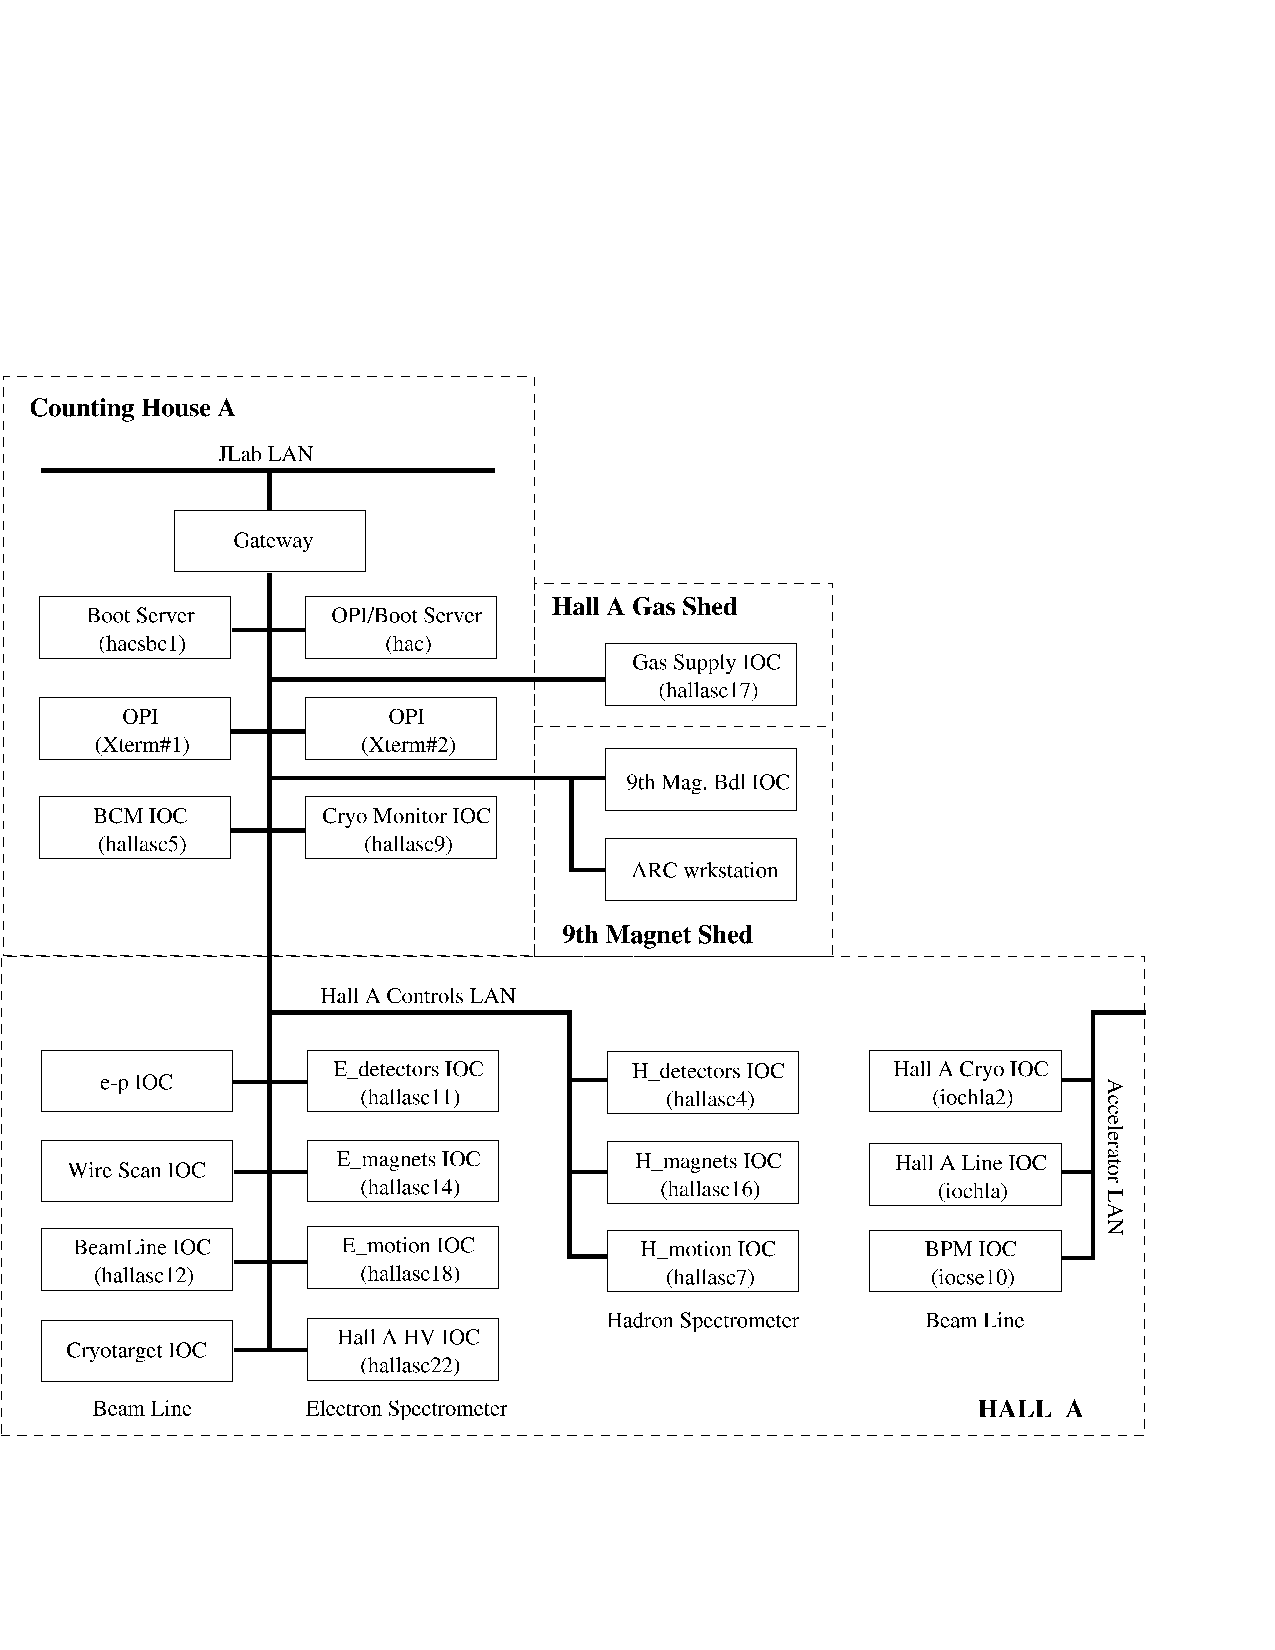
\includegraphics[angle=0,width=\textwidth]{HacOps_fig1_r}
{\linespread{1.}
\caption[Controls: Schematic]{Schematic of the Hall A controls
system.}
\label{fig:halla_controls}}
\end{center}
\end{figure}

Signal monitoring and command is performed by the IOCs. At the
heart of an IOC is a memory resident
database describing each of the signals to be monitored and controlled by the IOC.
Each database entry (record) corresponds to a signal. When a given record executes, it
accesses the appropriate I/O module to retrieve/update the signal value. The origin of this
record execution request can be local to the IOC
(i.e. another database record) or remote (i.e. operator intervention through an OPI or a
record located in another IOC).
In all cases, access to the record is by name and not by IOC location.
The general EPICS mechanism to access a record consists of
broadcasting the record name in the network.
Upon receiving the broadcast, every IOC in that network searches its database
to determine if it contains the record name being sought. The IOC holding the requested record
responds to the query establishing a connection with the querying process.

The interface provided by the IOCs to access their record database is geared towards efficiency and not
human friendliness. Two reasons dictate this choice: minimization of CPU overhead due to
interface management and the fact that the system is distributed.
Operator access to the record database of a given IOC is through a Graphical User interface (GUI)
process executing in a UNIX based computer.
The standard distribution of EPICS comes with a Motif based implementation of such GUI, the
so-called MEDM. It is possible to also implement a GUI to the IOCs using the Tool Command Language
(TCL) with X11 extensions (TK) (i.e. TCL/TK). Such implementation is used, for example, by the
Hall A cryotarget system.
There can be many instances of these GUIs executing in the same computer as well as in several
different computers
(i.e. the GUI processes are also distributed).
Each of these GUI processes can access multiple IOCs simultaneously and within each IOC,
all or a subset of the database records. The computers where these GUIs execute are referred to as the OPI.

\begin{figure}[htb]
\begin{center}
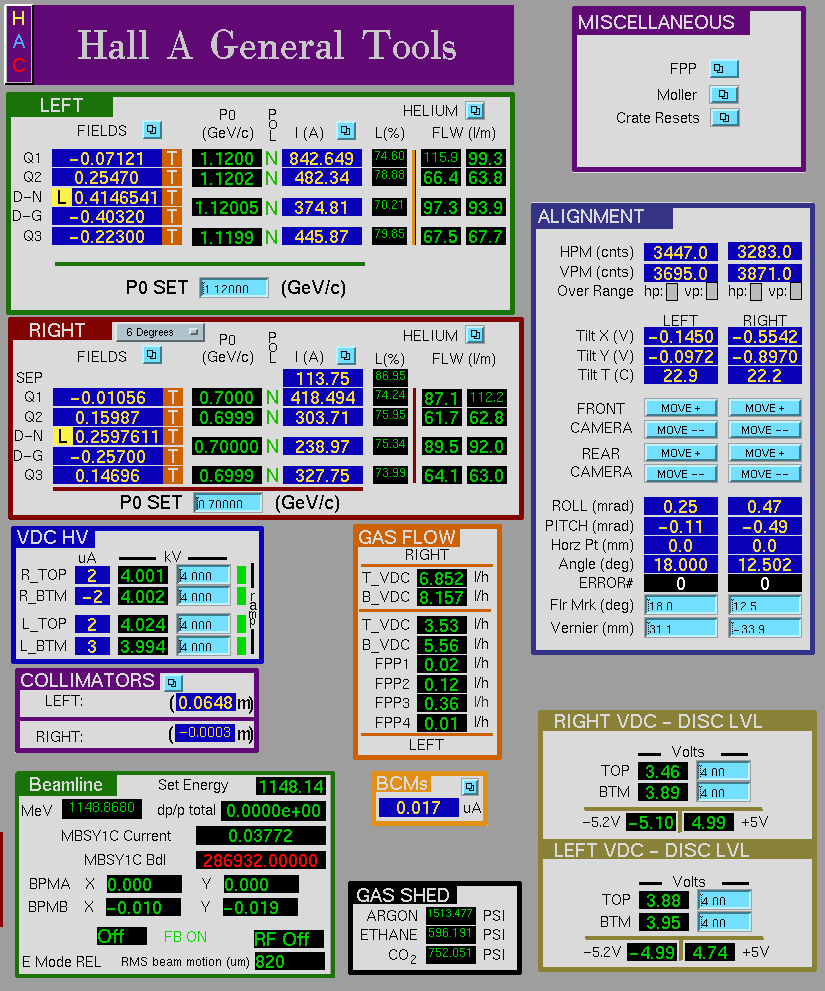
\includegraphics[angle=0,width=\textwidth]{medm_halla_tools}
{\linespread{1.}
\caption[Controls: Hall A Main Control Screen]{Hall A Main Control Screen.}
\label{fig:halla_screen}}
\end{center}
\end{figure}

Figure \ref{fig:halla_controls} shows a schematic view of the present Hall A controls layout.
Exchange of signals between Hall A and other JLab control systems takes place through the 
main Jefferson Lab network (JLab LAN). Presently, 
the system is in a state of flux as management
of various portions of the Hall A controls system is being transferred to the Accelerator 
Division Controls Group (ADCG). This might entail future changes
in the organization of the Hall A control
system like boot servers and IOC task re-arrangement. A brief
description of the present state of the system follows.

There are three IOCs in Hall A which at the present time are directly managed by the ADCG.
These IOCs are iocse10, iochla and iochla2. They are located in the row of racks next 
to the beam line. Iocse10 performs the readout of the Beam Position Monitors (BPMs)
located in Hall A (i.e. those located at Compton region and before the target).
Iochla handles Hall A beam line tasks like Fast Shut Down (FSD) logic,
M{\o}ller target motion, Beam Loss monitors and ionization chambers.
Hall A cryogenics distribution and magnet filling/level are controlled by iochla2
through a GPIB based network of CAMAC crates. This IOC also monitors all
spectrometer magnet temperatures during a magnet cooldown.
The iochla2 signals are available in the Hall A controls
network through a dedicated IOC (hallasc9) located in the electronics room (middle room) of the
Hall A Counting House.
Only Accelerator Operations personnel are allowed to reboot and/or perform any hardware/software changes in 
iocse10, iochla and iochla2 and the associated equipment that they control.
If necessary, hallasc9 can be rebooted by pressing the ``RESET'' push button located in the IOC front panel.
Such operation does not have any effect on the Hall A cryogenics distribution itself (hallasc9 does not
control any hardware, it is simply a signal repeater).
If a magnet cryogenics problem develops in Hall A, the Hall A on-call technical staff should be notified.

The controls layout of each High Resolution Spectrometer (HRS) is similar; each consists of three IOCs
which monitor and control the detector package infrastructure, general spectrometer functions 
and, spectrometer motion. In the case of the hadron HRS, these IOCs are hallasc4, hallasc16 and hallasc7. Hallasc4
and hallasc16 are located inside the detector hut. Hallasc4 is in the second floor of the detector electronics racks while
hallasc16 is located under the Box Beam supporting the detectors and detector electronics. Access to hallasc16 is
through a ``manhole''
located at the back of the detector hut. The IOC in charge of the hadron HRS
motion is located right at the back of the dipole (power supplies level). In the case of the electron HRS, the IOCs are
hallasc11, hallasc14 and hallasc18 respectively. Their location is similar to their hadron spectrometer counterparts.

The tasks assigned to IOCs hallasc7 and hallasc18 are well defined and unique: spectrometer motion.
Hallasc4 monitors/controls the Vertical Drift Chambers (VDCs) 
High Voltages (HV), discriminator threshold levels and the
low voltage power supplies for the discriminator cards as well as the Focal Plane Polarimeter
(FPP) tracking chamber's HVs, discriminator levels and 
low voltage power supplies.
Hallasc4 also controls the operation of the FPP carbon doors as
well as monitoring the gas flow to the FPP tracking
chambers and VDCs. In the case of the electron HRS, the corresponding IOC (hallasc11) monitors/controls similar quantities
for the VDCs only (there is no FPP system). The general spectrometer infrastructure IOCs (hallasc14 and hallasc16) monitor/control
magnets power supplies, field probes, hardware interlock systems and power leads cryogenic cooling, collimator motion,
magnet/spectrometer vacuum and spectrometer horizontal/vertical angles. If a problem arises, all these IOCs can be hardware
reset from the Hall A Counting House through the green buttons panel located in the middle room.

There is an extra IOC, hallasc22, located on the second floor of the electron HRS detector electronics racks 
(inside the detector hut). This IOC monitors and controls, through
a private network, various high voltage power supplies. Two of these supplies are located in the electron
HRS detector hut, one in the hadron HRS detector hut and one along the beam line. These power supplies are used by
various systems like the spectrometer scintillator planes (trigger), gas Cerenkov and Aerogel counters, electron HRS calorimeter,
FPP, hadron HRS calorimeter (when installed) and various
beam line systems like the ARC energy measurement system.

The beam line IOC hallasc12 is reserved, at this time, for Hall A application testing and development. There are other specific
purpose IOCs located in the group of electronics racks next to the beam line. The reader is referred to the specific description
of those systems and related instructions elsewhere in this OPS manual.

There are several Hall A controls related IOCs and computer systems outside the hall. Some of them are specific purpose
systems described elsewhere in this manual like the 9th magnet Bdl IOC and associated ARC workstation located inside the 9th magnet
shed, and they are described elsewhere in this manual. The others are briefly described below. 

Hallasc17 is located in the gas shed.
It monitors the supply of gas used by the tracking chambers (i.e. VDCs and FPP chambers).
If necessary, hallasc17 can be rebooted by pressing the ``RESET'' push button located in the IOC front panel.
Hallasc5 is located in the electronics room of the Hall A Counting House (middle room) in the same VME crate than hallasc9.
Hallasc5 monitors signals associated with Hall A beam current. It can be reset by pressing the ``RESET'' push button located in the
IOC front panel. The remaining computers and X-terminals associated with the Hall A controls are used as OPI and/or boot servers for the
IOCs. One of the X-terminals in the counting house is dedicated to the display of accelerator MEDM screens 
(it is automatic, no user involvement is required).

The ``hac'' computer is used to gain access to the Hall A control systems. Once logged into this computer, issue the command ``HAC\_hp''
if logging was accomplished through a Hewlett Packard computer console or ``HAC\_xt'' if through an X-terminal.
The Hall A controls main screen shown in Figure \ref{fig:halla_screen} will appear. Follow then the instructions given in the system of your interest.


\subsection{Personnel Responsible}
If a problem develops with the Hall A controls system, page J. Gomez at 849-7498. 

%\clearpage % forces LaTeX to finish all remaining open floats

% ===========  CVS info
% $Header: /group/halla/analysis/cvs/tex/osp/src/controls/HacOps.tex,v 1.2 2003/06/05 23:30:00 gen Exp $
% $Id: HacOps.tex,v 1.2 2003/06/05 23:30:00 gen Exp $
% $Author: gen $
% $Date: 2003/06/05 23:30:00 $
% $Name:  $
% $Locker:  $
% $Log: HacOps.tex,v $
% Revision 1.2  2003/06/05 23:30:00  gen
% Revision ID is printed in TeX
%
% Revision 1.1.1.1  2003/06/05 17:28:32  gen
% Imported from /home/gen/tex/OSP
%
%  Revision parameters to appear on the output
{\small
\begin{verbatim}CVS $Id: HacOps.tex,v 1.2 2003/06/05 23:30:00 gen Exp $\end{verbatim}
}
